To evaluate the performance of the \fullsys, we conducted several experiments in different energy conditions and with different event arrivals patterns. 
%
\subsection{Availability}
\begin{figure*}[t]
        \begin{subfigure}{.66\columnwidth}
            \includegraphics[width=\textwidth]{figures/sysAvailability}
                \caption{The \sys is powered by uncontrollable light sources---artificial light (night) and sunlight (day).}
            \label{fig:solarPwrCIS}
        \end{subfigure}\hfill
        \begin{subfigure}{.66\columnwidth}
            \includegraphics[width=\textwidth]{figures/rf_sysAvailability}
                \caption{The \sys is powered by an RF reader~\cite{r420_website} located 30-70\,cm aware from the RF tags (WISPs~\cite{smith_ubicomp_2006}).}
            \label{fig:rfPwrCIS}
        \end{subfigure}\hfill
        \begin{subfigure}{.66\columnwidth}
            \includegraphics[width=\textwidth]{figures/sysAvailability_artificial-light}
                \caption{The \sys is powered by a controllable array of LEDs in a dark room. \vspace{1em}}
            \label{fig:rfPwrCIS}
        \end{subfigure}
        \caption{Measuring \fullsys availability for a differed number of intermittent nodes. Generally, adding a node increases the system availability. This increment, however, is proportional to the \sys off-time.}
        \label{fig:pwrCIS}
\end{figure*} 
%
In Figure~\ref{fig:power_cycles} we showed that the power cycles of an RF- and solar-powered \sys are different, and therefore, we expected their on-times to be uniformly distributed, as modeled in Equation~\ref{eq:cisModel}. Here, we challenge our model and expection. 

Figure~\ref{fig:pwrCIS} shows the availability of three \sys{}s when they are powered by different energy sources (sunlight, artificial light, and RF) and for a different number of intermittent nodes.
The results clearly confim our expectation: when the power cycles are slightly different, the on-times are uniformly distributed. And they validate our model (the dashed lines represent the modeled availability when the nodes duty cycle is 15\%).

% We see that (i) the energy sources (sunlight, artificial light, and RF) power the \sys{}s intermittently, (ii) the \sys availability increases with number of nodes, and (iii) this addition is proportional to the \sys off-time. 
%
% The dashed lines represent Equation~\ref{eq:cisModel} expectation about the \sys availability for certain power cycles (10\% for the RF powered system, and 15\% for the light powered one). By comparing these lines to the measured ones we can conclude that these energy sources provide sufficient randomness to cause each node to have a slightly different power cycle which, in turn, causes their uptimes to be uniformly distributed in time.  

\subsection{Sensing}
\subsubsection{Experiment setup}
\label{sec:experiment_setup}
% \begin{figure}[t]
% 		\centering
% 		\includegraphics[width=\columnwidth]{figures/sysAvailability_artificial-light}
% 		\caption{\todo{can be removed, or merged with \sys availability figure with solar power or updated it and presented it} Implicit \fullsys' nodes distribution using artificial light power harvesting randomization}
% 		\label{fig:solarPwrCoIS}
% \end{figure} 

% \begin{figure}[t]
% 		\centering
% 		\includegraphics[width=\columnwidth]{figures/nodes_duty_cycles.eps}
% 		\caption{\fullcim nodes' duty cycles for a artificial light intensity ranges from $\approx 400$ to $\approx \SI{1000}{lux}$}
% 		\label{fig:solarPwrCoIS}
% \end{figure} 
%

%


% \paragraph{availability on a fine scale}
 % \todo{Because of the differences in intermittent nodes power cycles, their duty cycles are constantly shifting relative to each other ( Figure~\ref{fig:cisOntime}).  However, this study does zoom in on the \sys availability on short time scale and the effect of length of the differences between the nodes power cycles on the system short term availability. } 

After validating our observation on natural light and office artificial light, we designed a testbed with controllable light intensity for clarity and results reproducible. To this end, we blocked uncontrollable light sources with a box of $60 \times 40$\,cm. On the ceiling of the box, we attached a light strip of 2.5\,m with 150 LEDs that can produce 15 different light intensities. On the bottom of the box, we placed a \fullcim of 8 intermittent nodes (the hardware is described in Section~\ref{sec:hardware}).

The events in our experiments are spoken words (Table~\ref{tab:words}). We recorded different patterns of isolated words to emulate the arrival of bursts or individual events with varying inter-event and inter-bust timing. We used a Bluetooth speaker~\cite{jbl} to replay a certain record. The data were collected using logic anaylyzer~\cite{saleae} and processed on a laptop running Ubuntu 16.04 LTS. 


\subsubsection{Events detection rate}
%
\begin{figure}[t]
		\centering
	    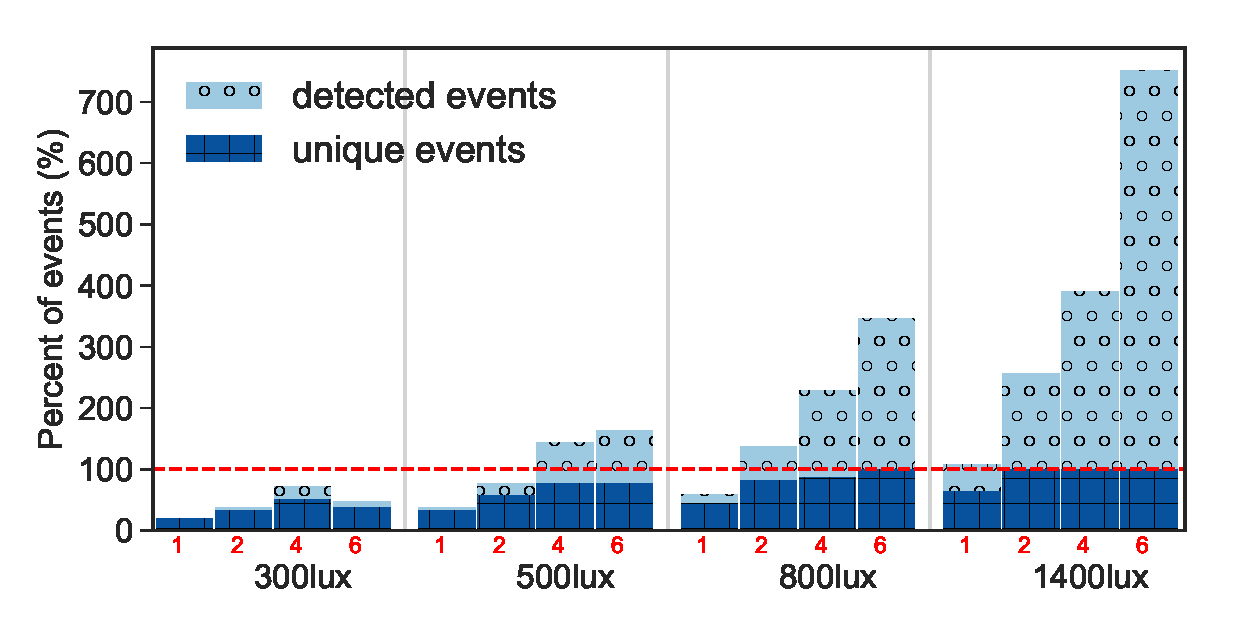
\includegraphics[width=\columnwidth]{figures/regular_events_capture_rate.eps}
		\caption{The number of detected and captured events by the \fullcim with eight intermittent nodes. The total number of external events is 240. In general, we see that when the light intensity increases, the number of detected and captured events rise too. Moreover, there is a positive correlation between the length of the inter-event arrival time and the detection and capture rates. Red numbers indicate events arrival interval.}
    	\label{fig:events_detection_rate}
\end{figure} 
These experiments show the total number of detected events and the number of uniquely detected ones with and without randomization. Also, they were conducted for a different type of events. 
%
\begin{figure}[t]
    \includegraphics[width=\columnwidth]{figures/events_burst_problem.pdf}
	\caption{When capturing a burst of events without randomized response, the majority of the nodes react to the first event of a burst and power down, missing the rest of the burst. Red numbers indicate events index in a burst.}
    \label{fig:events_burst_problem}
\end{figure}


\paragraph{Regular events}
\begin{figure}[t]
	\centering
     \includegraphics[width=\columnwidth]{figures/events_burst_rand}
    \caption{Response randomization enables a \sys to capture the entire burst of events with high capturing rates. It also reduces the number of duplicated events. Red numbers indicate events index in a burst.}
    \label{fig:events_burst_rand}
\end{figure}

Figure~\ref{fig:events_detection_rate} shows the percentage of the total captured events and the uniquely captured ones. In this experiment we vary the light intensity from $\SI{300}{lux}$ to $\SI{1400}{lux}$ and the inter-event time from $\SI{1}{sec}$ to $\SI{6}{sec}$. 

We clearly see a positive correlation between light intensity and the number of detected events. In particular, we see that the number of duplicated detected events rises dramatically when light intensity increases, demonstrating the overpowering problem. Moreover, increasing the inter-event arrival time also surges the number of duplicated events. The reason for this phenomenon is that when the time between events increases, the intermittent nodes sleep longer in low-power mode, and this reduces the inherent randomization of the intermittent nodes and leads them to the \textit{hibernating power state} (Section~\ref{sec:power_state}).  

Indirectly, these results show how a \sys can achieve a much higher duty cycle than its individual intermittent nodes: Figure~\ref{fig:cis_nodes_dutyCycle} shows that with a light intensity of $\SI{800}{lux}$ an intermittent node is active with a duty cycle of 30\% while Figure~\ref{fig:events_detection_rate} shows that a \sys of 8 nodes captures 100\% of the unique events when the time between them is \SI{6}{s}. 

\paragraph{Bursty events}
Figure~\ref{fig:events_burst_problem} shows the capturing behavior of a \sys when the events arrive in bursts. A burst of four events with one second between the individual events was fired every 20 seconds. Each burst was repeated 10 times and for four different light intensities. The nodes sleep in low-power mode when they finish processing, waiting for the next event. 

In general, we observe that the intermittent nodes react to the first event of a burst and power down shortly after missing other events in the burst. This results validate our theory about the side effect of the \textit{hibernating power state} (Section~\ref{sec:power_state}). These results also demonstrate the hibernating power problem on a wide range of power intensities, showing the significance of this problem. Next, we will show how randomized response can mitigate these problems. 

\subsubsection{Events detection rate with randomization}
\begin{table}
	\centering
    $
    \begin{array}{llll}\hline
     (lux,sec) & (800,6) & (1400,4) &(1400,6)\\\hline
    \text{randomization} &  205/432 & 236/675 & 223/493 \\
    \text{no randomization} & 240/831 &  240/938 & 240/1802 \\\hline
    \end{array}
    $
    \caption{Randomized response reduces the number of duplicated detected events,  when the \sys is overpowered, by 50\% while losing only 7\% of the unique events. The results are presented in the following format \textit{unique/total} detected events.}
    \label{tab:regular_rand}
\end{table}
%
\paragraph{Regular events} Table~\ref{tab:regular_rand} shows the number of detected events for three different scenarios. We see that randomized response reduces duplicated events by an average of $\approx$50\%, while only marginally lowers the number of the uniquely detected events. The intermittent nodes were responding to events with a probability of 65\% for the scenario of \SI{800}{lux} and \SI{6}{seconds} arrival time and the scenario of \SI{1400}{lux} and \SI{4}{seconds} arrival time. However, for the highest energy level and the longest inter-event arrival time a responding probability of 30\% was used.

\paragraph{Bursty events}
Figure~\ref{fig:events_burst_rand} shows that a \sys with randomized response spreads its resources--as compared to Figure~\ref{fig:events_burst_problem}--and captures the entire burst with a probability of above 90\%. We also observe a positive impact of randomized response when the system is under-powered ($\SI{500}{lux}$).

To randomize during bursty events, a node reacts with a certain probability on a event. This probability is different for each event since the node become active after the last recharge. In order to spread the nodes over the events, the probabilities need to increase for subsequent events, since some nodes have reacted already on previous events, and therefore the number of nodes still available is smaller after each event.
A node reacts with a probability of 40\% on the first event, with 50\% on the second event, 70\% on the third event and 100\% on the fourth event.
%40 50 70 100


\subsection{Coalesced intermittent command recognizer word detection accuracy}
\begin{table}[H]
\centering
\caption{Testing set}
\label{tab:words}
\begin{tabular}{lllll}
\hline
on    & off  & stop & clear & load   \\
go & pause & resume & edit  & cancel  \\  
\hline  
\end{tabular}
\end{table}

For evaluating the \fullcim accuracy, we used the word set in Table~\ref{tab:words}.
Each word was pronounced by a single speaker 20 times and recorded on a PC. One of these recordings was stored as a template on the \cim, while the remaining 19 were played back through a Bluetooth speaker~\cite{microphone} for testing.

The ratio between detected events and successfully recognized events per node is shown in Figure~\ref{fig:word_freq} and it averages out at  76.7\%. The difference between detection and capture is primarily caused by nodes that have insufficient buffered energy to finish recording.  

%
\begin{figure}
\centering
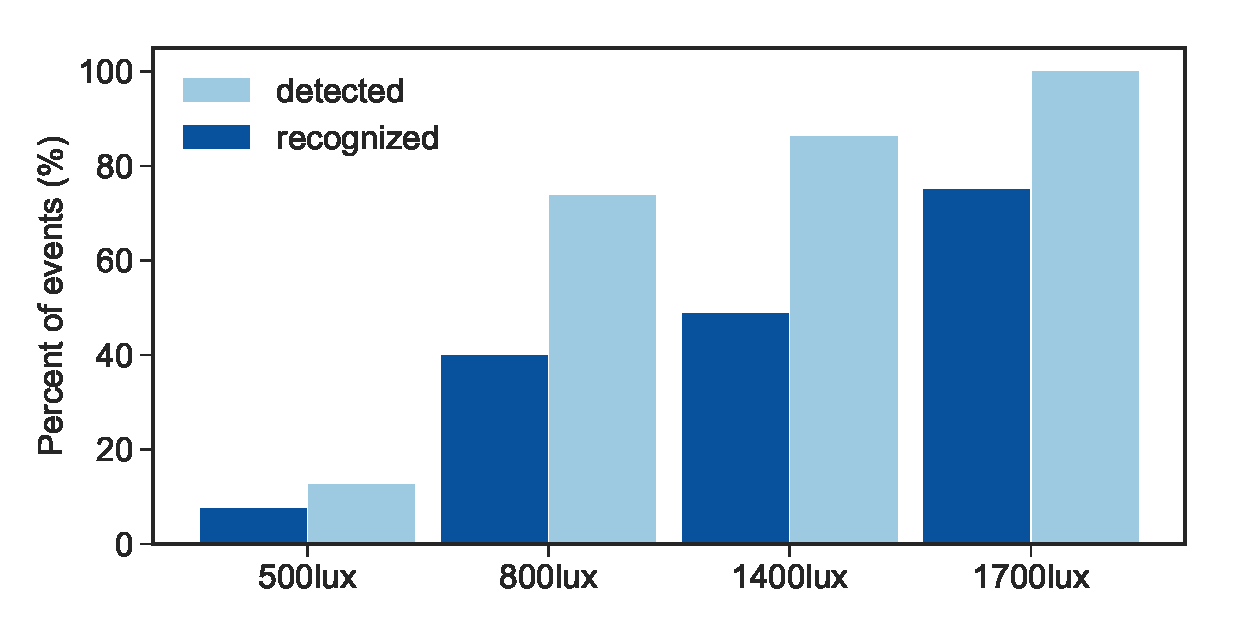
\includegraphics[width=\linewidth]{figures/detection_vs_recognition}
\caption{
% The percentage of successfully recognized words as compared to the detected ones.
Average number of successfully recognized words per node and average number of detected words per node, as percentages of the total number of played words. Words are relatively long events and therefore some of their recordings do not complete due to insufficient harvested energy.}
\label{fig:word_freq}
\end{figure}






